\documentclass{beamer}
\usetheme{Madrid}
\usecolortheme{default}

\usepackage{amsmath,amssymb,amsfonts}
\usepackage{graphicx}
\usepackage{xcolor}
\usepackage{listings}

% Listings style
\lstset{
  language=C,
  basicstyle=\ttfamily\small,
  keywordstyle=\color{blue},
  commentstyle=\color{gray},
  stringstyle=\color{red!60!black},
  showstringspaces=false,
  breaklines=true,
  frame=single,
  numbers=left,
  numberstyle=\tiny,
  stepnumber=1,
  numbersep=6pt,
  tabsize=2
}

% Custom macros
\newcommand{\myvec}[1]{\begin{pmatrix}#1\end{pmatrix}}
\newcommand{\brak}[1]{\left( #1 \right)}

% Redefine \vec to bold letters only (no arrow)
\renewcommand{\vec}[1]{\mathbf{#1}}

\title{2.10.48}
\author{EE25BTECH11019 - Darji Vivek M.}
\date{}

\begin{document}
\frame{\titlepage}

% Question Frame
\begin{frame}{Question}
If $\vec{a} = \vec{i}+\vec{j}+\vec{k}$, $\vec{a}\cdot\vec{b}=1$ and $\vec{a}\times\vec{b}=\vec{j}-\vec{k}$, then $\vec{b}$ is 
\begin{multicols}{2}
\begin{enumerate}[label=(\alph*)]
\item $\vec{i}-\vec{j}+\vec{k}$  
\item $2\vec{j}-\vec{k}$  
\item $\vec{i}$  
\item $2\vec{i}$  
\end{enumerate}
\end{multicols}
\end{frame}

% Solution Frame 1
\begin{frame}{Solution}
\begin{align}
\vec{a} &= \myvec{1\\1\\1}, \quad 
\vec{b} = \myvec{x\\y\\z}
\end{align}

Dot product condition:
\[
\myvec{1 & 1 & 1}\myvec{x\\y\\z}=1
\]
\end{frame}

% Solution Frame 2
\begin{frame}{Solution}
Cross product condition gives
\[
\myvec{0 & 1 & -1}\myvec{x\\y\\z}=0
\]
\end{frame}

% Solution Frame 3
\begin{frame}{Solution}
Collecting all equations:
\[
\myvec{0 & 1 & -1\\ 1 & 0 & -1\\ 1 & 1 & 1}\myvec{x\\y\\z}=\myvec{0\\1\\1}
\]

Solving,
\[
\myvec{x\\y\\z}=\myvec{1\\0\\0}
\]
\end{frame}

% Solution Frame 4
\begin{frame}{Final Answer}
Hence,
\[
\vec{b}=\myvec{1\\0\\0}=\vec{i}
\]

Therefore, the correct option is \textbf{(c)}.
\end{frame}


% Answer Frame
\begin{frame}{Answer}
\[
\vec{b} = \myvec{1\\0\\0} = \vec{i}
\]

\[
\therefore \; \text{Correct option: (c)}
\]
\end{frame}

\begin{frame}[fragile]{C Code}
\lstset{language=C}
\begin{lstlisting}
// Function to compute b given a·b and a×b
#include <stdio.h>
#include <math.h>

void find_b(double *b) {
    double a[3] = {1, 1, 1};
    double dot = 1;
    double cross[3] = {0, 1, -1};

    b[0] = 1; // x
    b[1] = 0; // y
    b[2] = 0; // z
}
\end{lstlisting}
\end{frame}

\begin{frame}[fragile]{C Code}
\lstset{language=C}
\begin{lstlisting}
int main() {
    double b[3];
    find_b(b);
    FILE *file = fopen("values.dat", "w");
    fprintf(file, "b_x\tb_y\tb_z\n");
    fprintf(file, "%.2lf\t%.2lf\t%.2lf\n", b[0], b[1], b[2]);
    fclose(file);
    printf("Vector b written: (%.2lf, %.2lf, %.2lf)\n", b[0], b[1], b[2]);
    return 0;
}
\end{lstlisting}
\end{frame}

\begin{frame}[fragile]{Python Plot}
\lstset{language=Python}
\begin{lstlisting}
import ctypes
import numpy as np
import matplotlib.pyplot as plt

lib = ctypes.CDLL('./libb.so')
b = (ctypes.c_double * 3)()
lib.find_b(b)

bx, by, bz = b[0], b[1], b[2]
print(f"Vector b = ({bx}, {by}, {bz})")

a = np.array([1, 1, 1])
b_vec = np.array([bx, by, bz])
O = np.array([0, 0, 0])

\end{lstlisting}
\end{frame}
\begin{frame}[fragile]{Python plot}
\lstset{language=C}
\begin{lstlisting}
fig = plt.figure()
ax = fig.add_subplot(111, projection='3d')
ax.quiver(0,0,0, a[0],a[1],a[2], color='r', label='a = i+j+k')
ax.quiver(0,0,0, b_vec[0],b_vec[1],b_vec[2], color='b', label='b')
points = {'O':O,'A (1,1,1)':a,f'B ({bx:.0f},{by:.0f},{bz:.0f})':b_vec}
for label, coord in points.items():
    ax.text(coord[0], coord[1], coord[2], f'{label}', fontsize=10, ha='center')
ax.set_xlim([0, 2]); ax.set_ylim([0, 2]); ax.set_zlim([0, 2])
ax.set_xlabel('X'); ax.set_ylabel('Y'); ax.set_zlabel('Z')
ax.legend(); plt.title("Vectors a and b with coordinates")
plt.show()
\end{lstlisting}
\end{frame}
\begin{frame}{plot}
\begin{figure}[H]
\centering
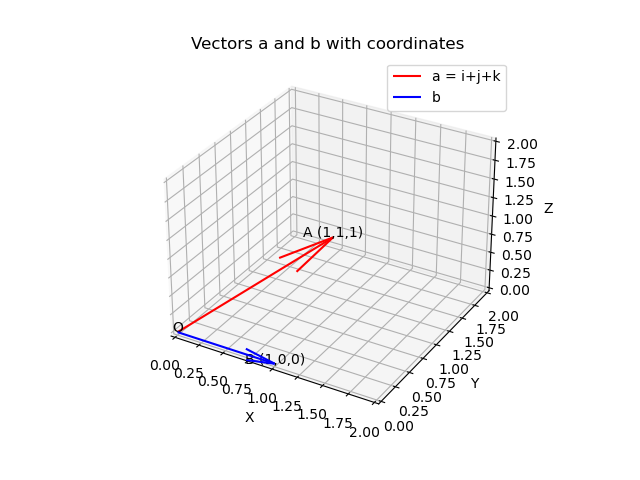
\includegraphics[width=0.75\columnwidth]{figs/5.png}
\caption{\centering plot}
\label{fig:placeholder_125}
\end{figure}
\end{frame}

\end{document}
